\chapter{Derivatives}
\label{app:derivatives}

\section{Derivative of Cross Product}
\label{sec:app_d_cross_product}
The derivative of a cross product can be calculated analogue to matrix derivatives.
The skew symmetric cross matrix is
\begin{equation}
\mathbf{a}^\times = \left[
\begin{array}{ccc}
0 & -a_3 & a_2 \\
a_3 & 0 & -a_1 \\
-a_2 & a_1 & 0
\end{array} \right]
\end{equation}
and the appropriate derivatives are therefore
\begin{equation}
\frac{\partial}{\partial \mathbf{a}} \left( \mathbf{a} \times \mathbf{b} \right)
= - \mathbf{b}^\times
\end{equation}
and
\begin{equation}
\frac{\partial}{\partial \mathbf{a}} \left( \mathbf{b} \times \mathbf{a} \right)
=  \mathbf{b}^\times
\end{equation}

\section{Derivative w.r.t. Gibbs-Rodriquez Parameters}
\label{sec:app_dwrt_rodriquez}
Derivative of the rotation matrix \cref{eq:rod_to_C} w.r.t. the Gibbs-Rodriquez parameter:

\begin{equation*}
\frac{\partial \mathbf{C}}{\partial \lambda_1} = 
\left(\begin{array}{ccc} 
\frac{4\, {\lambda_1}\, \left({{\lambda_2}}^2 + {{\lambda_3}}^2\right)}{\nu}^2 & 
\frac{2\, {\lambda_2}}{\nu} + \frac{4\, {\lambda_1}\, {\lambda_3} - {\lambda_1}\, {\lambda_2}}{\nu^2} & 
\frac{2\, {\lambda_3}}{\nu} - \frac{4\, {\lambda_1}\, \left({\lambda_2} + {\lambda_1}\, {\lambda_3}\right)}{\nu^2}\\ 
\frac{2\, {\lambda_2}}{\nu} - \frac{4\, {\lambda_1}\, \left({\lambda_3} + {\lambda_1}\, {\lambda_2}\right)}{\nu^2} & 
\frac{4\, {\lambda_1}\, \left({{\lambda_1}}^2 + {{\lambda_3}}^2\right)}{\nu^2} - \frac{4\, {\lambda_1}}{\nu} &
\frac{4\, {\lambda_1}\, \left({\lambda_1} - {\lambda_2}\, {\lambda_3}\right)}{\nu^2} - \frac{2}{\nu}\\
\frac{2\, {\lambda_3}}{\nu} + \frac{4\, {\lambda_1}\, \left({\lambda_2} - {\lambda_1}\, {\lambda_3}\right)}{\nu^2} &
\frac{2}{\nu} - \frac{4\, {\lambda_1}\, \left({\lambda_1} + {\lambda_2}\, {\lambda_3}\right)}{\nu^2} & \frac{4\, {\lambda_1}\, \left({{\lambda_1}}^2 + {{\lambda_2}}^2\right)}{\nu^2} - \frac{4\, {\lambda_1}}{\nu}
\end{array}\right)
\end{equation*}

\begin{equation*}
\frac{\partial \mathbf{C}}{\partial \lambda_2} = 
\left(\begin{array}{ccc} 
\frac{4\, {\lambda_2}\, \left({{\lambda_2}}^2 + {{\lambda_3}}^2\right)}{{\nu}^2} - \frac{4\, {\lambda_2}}{\nu} &
\frac{2\, {\lambda_1}}{\nu} + \frac{4\, {\lambda_2}\, \left({\lambda_3} - {\lambda_1}\, {\lambda_2}\right)}{{\nu}^2} &
\frac{2}{\nu} - \frac{4\, {\lambda_2}\, \left({\lambda_2} + {\lambda_1}\, {\lambda_3}\right)}{{\nu}^2}\\
\frac{2\, {\lambda_1}}{\nu} - \frac{4\, {\lambda_2}\, \left({\lambda_3} + {\lambda_1}\, {\lambda_2}\right)}{{\nu}^2} &
\frac{4\, {\lambda_2}\, \left({{\lambda_1}}^2 + {{\lambda_3}}^2\right)}{{\nu}^2} & \frac{2\, {\lambda_3}}{\nu} + \frac{4\, {\lambda_2}\, \left({\lambda_1} - {\lambda_2}\, {\lambda_3}\right)}{{\nu}^2}\\
\frac{4\, {\lambda_2}\, \left({\lambda_2} - {\lambda_1}\, {\lambda_3}\right)}{{\nu}^2} - \frac{2}{\nu} &
\frac{2\, {\lambda_3}}{\nu} - \frac{4\, {\lambda_2}\, \left({\lambda_1} + {\lambda_2}\, {\lambda_3}\right)}{{\nu}^2} &
\frac{4\, {\lambda_2}\, \left({{\lambda_1}}^2 + {{\lambda_2}}^2\right)}{{\nu}^2} - \frac{4\, {\lambda_2}}{\nu} \end{array}\right)
\end{equation*}

\begin{equation*}
\frac{\partial \mathbf{C}}{\partial \lambda_3} = 
\left(\begin{array}{ccc} \frac{4\, {\lambda_3}\, \left({{\lambda_2}}^2 + {{\lambda_3}}^2\right)}{{\nu}^2} - \frac{4\, {\lambda_3}}{\nu} & \frac{4\, {\lambda_3}\, \left({\lambda_3} - {\lambda_1}\, {\lambda_2}\right)}{{\nu}^2} - \frac{2}{\nu} & \frac{2\, {\lambda_1}}{\nu} - \frac{4\, {\lambda_3}\, \left({\lambda_2} + {\lambda_1}\, {\lambda_3}\right)}{{\nu}^2}\\ \frac{2}{\nu} - \frac{4\, {\lambda_3}\, \left({\lambda_3} + {\lambda_1}\, {\lambda_2}\right)}{{\nu}^2} & \frac{4\, {\lambda_3}\, \left({{\lambda_1}}^2 + {{\lambda_3}}^2\right)}{{\nu}^2} - \frac{4\, {\lambda_3}}{\nu} & \frac{2\, {\lambda_2}}{\nu} + \frac{4\, {\lambda_3}\, \left({\lambda_1} - {\lambda_2}\, {\lambda_3}\right)}{{\nu}^2}\\ \frac{2\, {\lambda_1}}{\nu} + \frac{4\, {\lambda_3}\, \left({\lambda_2} - {\lambda_1}\, {\lambda_3}\right)}{{\nu}^2} & \frac{2\, {\lambda_2}}{\nu} - \frac{4\, {\lambda_3}\, \left({\lambda_1} + {\lambda_2}\, {\lambda_3}\right)}{{\nu}^2} & \frac{4\, {\lambda_3}\, \left({{\lambda_1}}^2 + {{\lambda_2}}^2\right)}{{\nu}^2} \end{array}\right)
\end{equation*}
where
\begin{equation*}
\nu = {\lambda_1}^2 + {\lambda_2}^2 + {\lambda_3}^2 + 1
\end{equation*}


%\section{Derivative w.r.t. Inertia Tensor A}
%XXX derivative w.r.t inertia tensor components (and it's inverse)

%\section{Derivative w.r.t. Inertia Tensor B}
%XXX derivative w.r.t diagonal inertia tensor and rotation matrix (and it's inverse)

\chapter{Additional Plots}

\section{Sensor Specification}
\begin{figure}[hbtp]
\centering
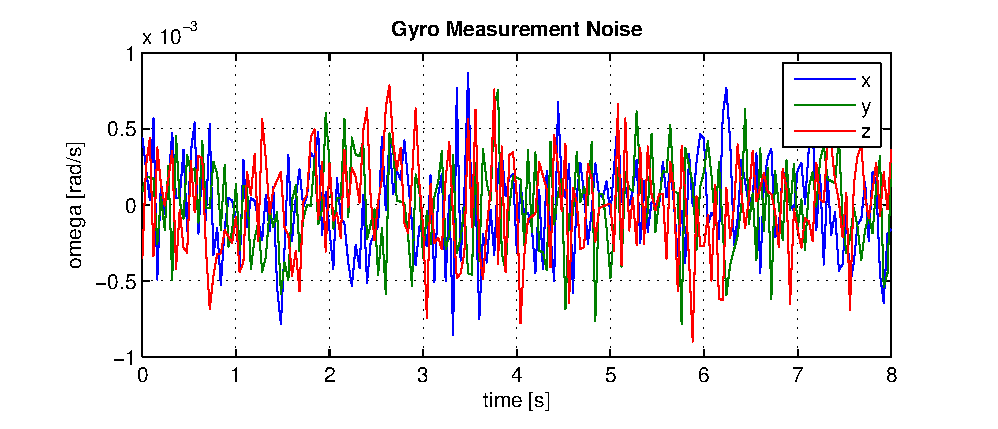
\includegraphics[width = \textwidth]{images/appendix/gyro_noise.eps}
\caption{Measurement noise of MPU-6000 gyro. The RMS error is about $3.2 \cdot 10^{-4} rad/s$.}
\label{fig:gyro_noise}

\end{figure}
\begin{figure}[hbtp]
\centering
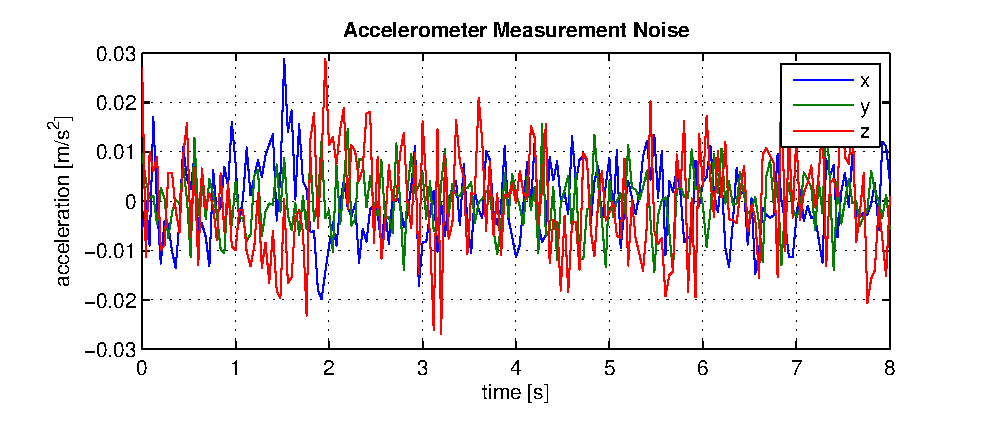
\includegraphics[width = \textwidth]{images/appendix/accel_noise.eps}
\caption{Measurement noise of MPU-6000 accelerometer. The RMS error is about $8.2 \cdot 10^{-3} m/s^2$.}
\label{fig:accel_noise}
\end{figure}



\section{Actuation Unit Position Estimate Variance}
\begin{figure}[hbtp]
\centering
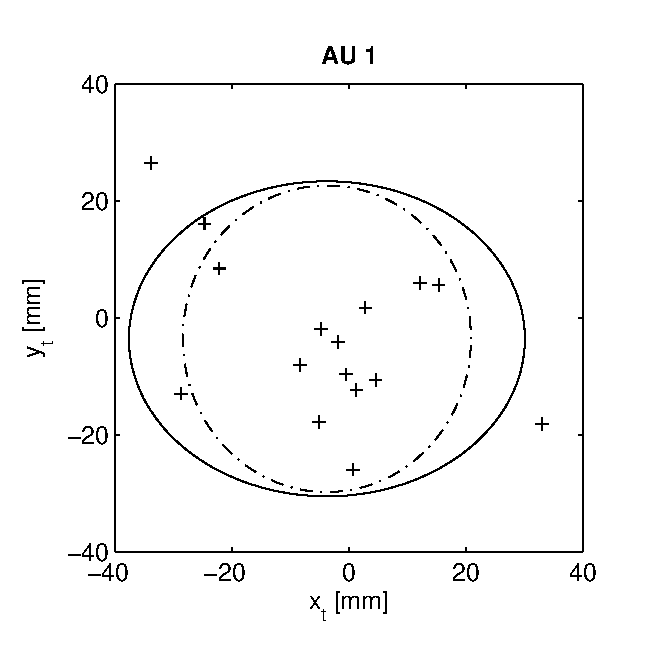
\includegraphics[width = 0.45\textwidth]{images/results/confidence_95_interval_AU1.eps}
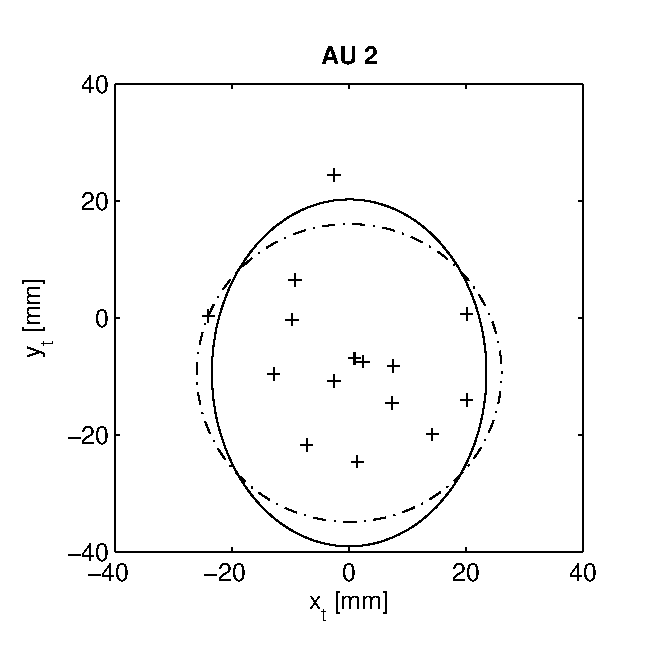
\includegraphics[width = 0.45\textwidth]{images/results/confidence_95_interval_AU2.eps} \\
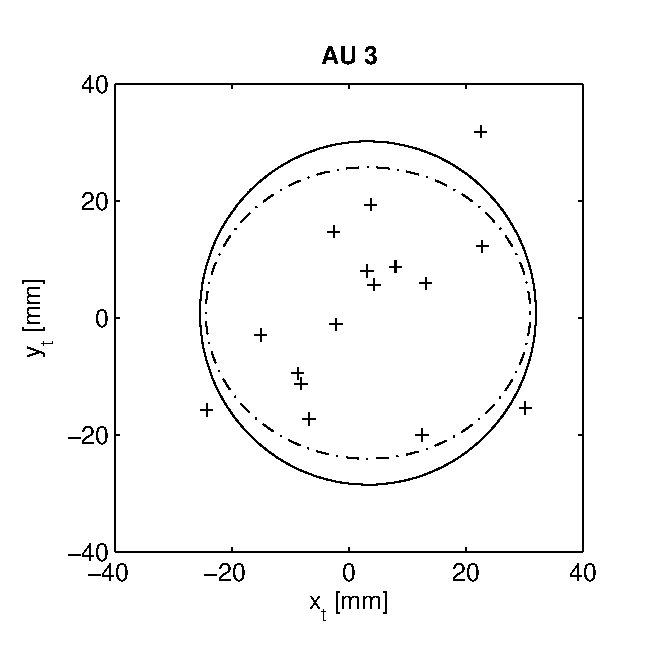
\includegraphics[width = 0.45\textwidth]{images/results/confidence_95_interval_AU3.eps}
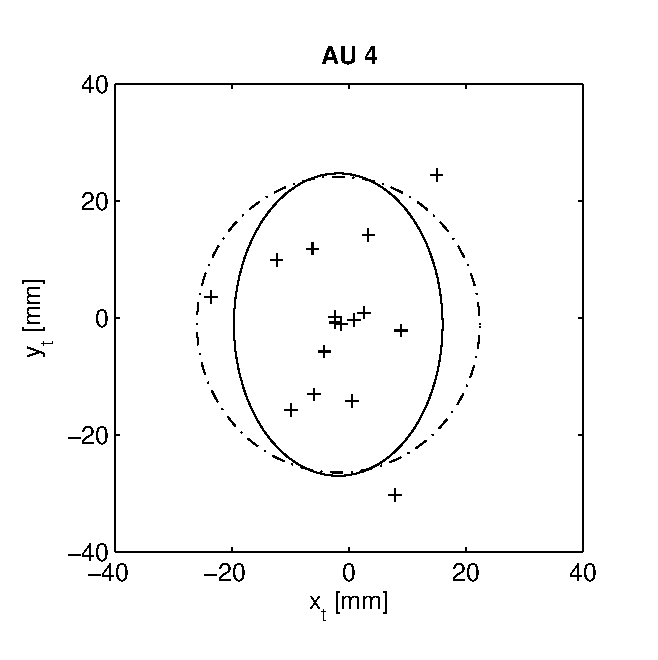
\includegraphics[width = 0.45\textwidth]{images/results/confidence_95_interval_AU4.eps}
\caption{Distribution of actuator position estimates. 16 datasets with 24 input vectors each and one sample per input vector.
$\mathbf{+}$ represent the results used to measure the variance.
\textbf{dashed}: 95\% confidence interval calculated from covariance matrix.
\textbf{solid}: 95\% confidence interval calculated from multiple results. }
\label{fig:result_95pc_confidence_all}
\end{figure}


\section{Parameter Estimates}
\label{sec:app_parameter_est}

\begin{table}[H]
\begin{tabular}{lcrrrc}
Variable & Parameter & Mean & Std1 & Std2 & Unit \\
\hline \hline
AU 1 Orientation & $\lambda_1^1$ & -1.741915837 & 0.009166579 & 0.012530239 & $[-]$ \\
                 & $\lambda_1^1$ & -0.176579713 & 0.002681883 & 0.004968607 & $[-]$ \\
                 & $\lambda_1^1$ & 0.305726308 & 0.005847842 & 0.005828741 & $[-]$ \\
AU 2 Orientation & $\lambda_1^2$ & 1.731130287 & 0.009248668 & 0.012420543 & $[-]$ \\
                 & $\lambda_1^2$ & -0.175376215 & 0.004405455 & 0.005072152 & $[-]$ \\
                 & $\lambda_1^2$ & -0.30558795 & 0.005344155 & 0.006040389 & $[-]$ \\
AU 3 Orientation & $\lambda_1^3$ & 0.000591361 & 0.003007073 & 0.003001555 & $[-]$ \\
                 & $\lambda_1^3$ & -0.177077214 & 0.001937974 & 0.003373292 & $[-]$ \\
                 & $\lambda_1^3$ & 6.49754E-05 & 0.001885305 & 0.00219974 & $[-]$ \\
AU 4 Orientation & $\lambda_1^3$ & -0.000792178 & 0.001775381 & 0.003710602 & $[-]$ \\
                 & $\lambda_1^3$ & 1.001931526 & 0.003799805 & 0.005906192 & $[-]$ \\
                 & $\lambda_1^3$ & -0.000526266 & 0.001774314 & 0.003620448 & $[-]$ \\
\hline
Inertia Tensor & $J_1$ & 14.57403705 & 0.023883239 & 0.036148512 & kg m$^2$ \\
               & $J_2$ & 15.56447564 & 0.021928529 & 0.037834855 & kg m$^2$ \\
               & $J_3$ & 15.47542575 & 0.034973044 & 0.039080129 & kg m$^2$ \\
               & $J_4$ & 0.071671104 & 0.024527294 & 0.021029481 & kg m$^2$ \\
               & $J_5$ & 0.215309911 & 0.017266071 & 0.020303492 & kg m$^2$ \\
               & $J_6$ & 0.046880029 & 0.008459791 & 0.019904439 & kg m$^2$ \\
\hline
Center of Gravity & $\mathbf{p}_{b,x}^{cob,cog}$ & -0.000101592 & 0.00011136 & 0.000153066 & m \\
                  & $\mathbf{p}_{b,y}^{cob,cog}$ & -2.53771E-05 & 0.000150175 & 0.00014934 & m \\
                  & $\mathbf{p}_{b,z}^{cob,cog}$ & -3.00404E-06 & 9.90231E-05 & 0.000147795 & m \\
\hline
\end{tabular}
\caption{Optimization result of the parameters as defined in \cref{sec:parameterization}, \cref{tab:params_updated} for simulation data. Results have been calculated for 16 distinct datasets. \textbf{Mean} is the mean parameter estimate of the samples with standard deviation \textbf{Std1}. The mean over the expected standard deviation from the optimization residual is given as \textbf{Std2}.}
\end{table}

\begin{table}[H]
\begin{tabular}{lcrrrc}
Variable & Parameter & Mean & Std1 & Std2 & Unit \\
\hline \hline
AU 1 Orientation & $\lambda_1^1$ & -1.841689724 & 0.038953292 & 0.046525688 & $[-]$ \\
                 & $\lambda_2^1$ & -0.252614018 & 0.013382649 & 0.015530261 & $[-]$ \\
                 & $\lambda_3^1$ &  0.26987087 & 0.016083825 & 0.01614782 & $[-]$ \\
AU 2 Orientation & $\lambda_1^2$ &  1.726674693 & 0.033042682 & 0.04142205 & $[-]$ \\
                 & $\lambda_2^2$ & -0.017593159 & 0.01355598 & 0.012474474 & $[-]$ \\
                 & $\lambda_3^2$ & -0.335327836 & 0.018041183 & 0.021212657 & $[-]$ \\
AU 3 Orientation & $\lambda_1^3$ & -0.010025281 & 0.007923151 & 0.009106036 & $[-]$ \\
                 & $\lambda_2^3$ & -0.182941004 & 0.00930763 & 0.011412447 & $[-]$ \\
                 & $\lambda_3^3$ & -0.006427754 & 0.005374822 & 0.004353904 & $[-]$ \\
AU 4 Orientation & $\lambda_1^4$ & -0.103928184 & 0.008785253 & 0.009708355 & $[-]$ \\
                 & $\lambda_2^4$ &  0.984826536 & 0.016823497 & 0.020915549 & $[-]$ \\
                 & $\lambda_3^4$ & -0.096597351 & 0.009209886 & 0.010746297 & $[-]$ \\
\hline
Inertia Tensor & $J_1$ & 14.70897958 & 0.135567324 & 0.26947353 & kg m$^2$ \\
               & $J_2$ & 17.21843941 & 0.175921877 & 0.328509894 & kg m$^2$ \\
               & $J_3$ & 16.40495373 & 0.168460164 & 0.415076368 & kg m$^2$ \\
               & $J_4$ & 0.511843681 & 0.135145759 & 0.136563542 & kg m$^2$ \\
               & $J_5$ & -0.05958936 & 0.126076425 & 0.145986446 & kg m$^2$ \\
               & $J_6$ & 0.234369497 & 0.126702251 & 0.134153298 & kg m$^2$ \\
\hline
Center of Gravity & $\mathbf{p}_{b,x}^{cob,cog}$ & 0.000495015 & 0.00028417 & 0.00026949 & m \\
                  & $\mathbf{p}_{b,y}^{cob,cog}$ & -0.000705644 & 0.000267855 & 0.000228525 & m \\
                  & $\mathbf{p}_{b,z}^{cob,cog}$ & -0.000215293 & 0.000317137 & 0.000338427 & m \\
\hline
\end{tabular}
\caption{Optimization result of the parameters as defined in \cref{sec:parameterization}, \cref{tab:params_updated} for real data. Results have been calculated for 16 distinct datasets. \textbf{Mean} is the mean parameter estimate of the samples with standard deviation \textbf{Std1}. The mean over the expected standard deviation from the optimization residual is given as \textbf{Std2}. }
\end{table}
